%!TEX root = /Users/stwaidele/Dropbox (Leisinger)/02 - AKAD/Projektbericht/Möglichkeiten der Digitalen Kontaktaufnahme im Endkundenbereich/vorlage.tex

\section{Grundlagen} % (fold)
\label{sec:grundlagen}

\subsection{Digitale Kontaktaufnahme} % (fold)
\label{sub:digitale_kontaktaufnahme}

Der Begriff \buzz{digitale Kontaktaufnahme} beschreibt im Rahmen dieser Arbeit den Vorgang der ersten Interaktion, die zwischen einem Kunden und einem Unternehmen mit Hilfe von digitalen Medien statt findet. Sie stellt daher einen \buzz{Medienbruch} dar, welcher im beidseitigen Interesse möglichst einfach und reibungslos für den Kunden verlaufen sollte. 

Für das Unternehmen ist es wichtig, dass der Wechsel des Kontaktmediums zielgerichtet und treffsicher auf das digitale Angebot des Betriebs leitet. Nur so können Streuverluste bzw. verlustbehaftete Umwege über Drittanbieter\footnote{etwa Buchungsplattformen (Buchungsprovisionen) oder Suchmaschinen (Anzeige von Konkurrenten)} vermieden werden.

Die digitale Kontaktaufnahme ist somit Startpunkt von Prozessen oder Teilprozessen, die mit Hilfe von digitalen Kommunikationsmitteln durchgeführt werden.
% subsection digitale_kontaktaufnahme (end)

\subsection{Kunden} % (fold)
\label{sub:kunden}

Für die Zwecke dieser Untersuchung soll ein sehr weit gefasster Kundenbegriff zum Einsatz kommen, der Interessenten und potentielle Interessenten einschließt. Jedoch soll die Voraussetzung gelten, dass bereits ein nicht--digitaler Kontakt mit dem Unternehmen zu Stande gekommen ist. Dies kann durch den tatsächlichen Besuch des Betriebs, aber auch durch Prospekte, Plakate oder Informationstafeln geschehen sein.
% subsection kunden (end)

\subsection{Notwendigkeit des Medienbruchs} % (fold)
\label{sec:medienbruch}

Bei Betrachtung eines vor Ort anwesenden Kundens stellt der Wechsel des Kommunikationskanals auf ein digitales Medium einen teilweisen Rückschritt dar. Der unmittelbare Kontakt zum Servicemitarbeiter geht zunächst verloren und wird zumindest durch mittelbare Kommunikation und teilweise sogar durch die Wiedergabe unpersönlich hinterlegter Informationen ersetzt.
Betrachtet man jedoch die vielen Situationen, in denen ein Gast zwar vor Ort ist, aber keinen direkten Kontakt zum Servicepersonal hat, so können digital hinterlegte bzw. dynamisch generierte Informationen dem Gast einen deutlichen Mehrwert gegenüber gedruckten Materialien bieten.

Im Jahr 2013 haben 36\% der Reisenden mit mobilem Internetzugang während ihrer Urlaubsreise im Web 2.0 Beiträge veröffentlicht.\footnote{vgl. \cite{reiseanalyse}, Seite 5} Der Urlauber ist somit „sowohl Nutzer als auch Quelle von Informationen“.\footnote{\cite{reiseanalyse}, Seite 5} Daher ist es für touristische Betriebe wünschenswert, diesen Informationsfluss positiv zu beeinflussen. Der zumindest teilweise Wechsel des Kommunikationskanals schafft die Voraussetzungen dafür.
% subsection notwendigkeit_des_medienbruchs (end)
% section grundlagen (end)

\newpage
\section{Tourismus und Gastgewerbe} % (fold)
\label{sec:tourismusbranche}

\subsection{Begriffsbestimmung} % (fold)
\label{sub:begriffsbestimmung}
Der Tourismus beschäftigt sich mit Erscheinungen und Beziehungen, die mit dem Verlassenen des üblichen Lebensmittelpunkt und dem vorübergehenden Aufenthalt in einer anderen Region verbunden sind.\footnote{vgl. \cite{gabler:tourismus}}

Das Gastgewerbe ist die Untermenge der touristischen Betriebe, welche sich mit der Unterbringung und Verpflegung von Reisenden befasst. Der Deutsche Hotel– und Gaststättenverband\acused{DeHoGa} (\ac{DeHoGa}) gliedert das Gastgewerbe in Hotellerie, sonstige Beherbergungsbetriebe, speisegeprägte Gastronomie, getränkegeprägte Gastronomie sowie Caterer.\footnote{vgl. \cite{dehoga:zahlenspiegel}, Seite 1} Eine grobe Einteilung ist somit in Beherbergung, d.h. die Möglichkeit des Übernachtens gegen Bezahlung für einen kurzen Zeitraum, und Gastronomie, d.h. das Angebot von Speisen und Getränken zum sofortigen Verzehr, möglich.\footnote{vgl. \cite{destatis:gastgewerbe}}

Speziell die Gäste der Getränke-- aber auch die Speisegastronomie fallen nicht unter die oben genannte Definition von Tourismus nach Gabler, da diese Betriebe durchaus auch am Ort des üblichen Lebensmittelpunkts besucht werden. Da diese Unterscheidung auch in den Veröffentlichungen des Statistischen Bundesamts und des \ac{DeHoGa}\footnote{z.B. \cite{dehoga:zahlenspiegel}} nicht zu tragen kommt, soll dies auch im Rahmen dieser Arbeit nicht berücksichtigt werden.
% subsection begriffsbestimmung (end)

\subsection{Generelle Betrachtung des Gastgewerbes} % (fold)
\label{sec:generelltouri}
Wie schon aus den Definitionen hervorgeht, umfasst das Gastgewerbe ein Vielzahl von Betriebsarten, die sich in Größe, Betriebsstruktur, Qualitäts– sowie Preisniveau und Umsatzstärke deutlich von einander unterscheiden. Zum Gastgewerbe zählt die Imbissbude, die vom Inhaber alleine betrieben wird, das Sternerestaurant mit großer Küchen– und Servicebrigarde, der Wohnmobilstellplatz am Stadtrand und auch das 5–Sterne Grandhotel in bester Lage.

Eine Gemeinsamkeit verbindet jedoch diese Betriebstypen: Die typischen Mitarbeiter sind in der Regel wenig technikaffin. Für die Leistungserstellung wird zwar Technik benötigt, diese wird jedoch vom Personal lediglich bedient und nicht eingerichtet.\footnote{z.B. Buchungssysteme, Registrierkassen oder auch programmierbare Öfen} Die Servicemitarbeiter sind im direkten Kundenkontakt begabt und geschult, die Küchenmitarbeiter hingegen erstellen ihre Leistung meist ohne Kundenkontakt. Bei beiden Gruppen gehören Fähigkeiten der digitalen Kommunikation mit den Kunden nicht zum Anforderungsprofil.\\
Eine Ausnahme bilden hier die Mitarbeiter der Hotelrezeption bzw. Bankettabteilung von entsprechenden Betrieben. In diesen Bereichen ist die schriftliche Kommunikation mit Interessenten und Kunden durchaus üblich, welche heute überwiegend per E–Mail abgewickelt wird. 
Spezialisierte Mitarbeiter in den Bereichen IT oder Marketing findet man erst in Betrieben von deutlich überdurchschnittlicher Größe. 

Das Angebot der Betriebe ist häufigen und oftmals auch kurzfristigen Schwankungen unterworfen. Diese reichen von der Anpassung der Zimmerpreise zum Saisonwechsel, über Aktionangebote oder Tageskarten in Restaurants bis hin zur plötzlichen Nichtverfügbarkeit von Artikeln aufgrund von hoher Nachfrage. Die Entscheidungen hierüber können auf unterschiedlichen Hierarchieebenen und in verschiedenen Abteilungen getroffen werden. Geschäftsprozesse sind in der Regel kaum integriert und weisen Medienbrüche auf.\footnote{vgl. \cite{waidele:integration}, Seite 10ff} Hierdurch entstehen Herausforderungen für die digitale Kommunikation, die bei der Auswahl der Kontaktmöglichkeiten beachtet werden müssen.
% subsection generelle_betrachtung_des_gastgewerbes (end)

\subsection{Betriebsgrößen nach Umsatzgröße} % (fold)
\label{sub:betriebsgrossen_nach_umsatzgrosse}
Der durchschnittliche Jahresumsatz der 247.949 gastgewerblichen Betriebe betrug 2012 etwas mehr als 285.000€.\footnote{vgl. \cite{destatis:genesis}} Hierbei ist jedoch die statistische Verteilung nicht gleichmäßig. So erwirtschafteten 11\% der Betriebe\footnote{Hierzu gehören viele Hotel– oder Restaurantketten, wodurch dies 5\% der Unternehmen entspricht} über die Hälfte des gesamten Umsatzes.

\begin{table}[H]
\begin{center}
\begin{footnotesize}
\begin{tabular}{| l | r | r  r | r |}  \hline                       
  \textbf{Umsatzgrößenklasse}            & \textbf{Betriebe} & \multicolumn{2}{|l|}{\textbf{Umsatz}}  & \textbf{ø pro Betrieb} \\ \hline 
  unter 100.000 €               & 98.067   &  4.955.000 € &   (7\%) &    50.522 € \\  \hline  
  100.000 € bis unter 200.000 € & 54.619   &  6.804.000 € &  (10\%) &   124.572 € \\  \hline  
  200.000 € bis unter 500.000 € & 48.982   & 13.008.000 € &  (18\%) &   265.567 € \\  \hline  
  500.000 € bis unter 1 Mill. € & 18.060   &  9.004.000 € &  (13\%) &   500.775 € \\  \hline  
  1 Mill. € und mehr            & 28.212   & 36.762.000 € &  (52\%) & 1.303.063 € \\  \hline  
  \textbf{Summe}                         & 247.949  & 70.573.000 € & (100\%) &   284.627 € \\  \hline  
\end{tabular}
\end{footnotesize}
\caption[Einteilung gastgewerblicher Betriebe nach Umsatz]{Einteilung gastgewerblicher Betriebe nach Umsatz\protect\footnotemark}
\label{tab:betriebsgroessen}
\end{center}
\end{table}
\footnotetext{Datenbasis \cite{destatis:genesis}, Prozent– und Durchschnitswerte eigene Berechnung}
% subsection betriebsgrossen_nach_umsatzgrosse (end)

\subsection{Kleine Betriebe im Gastgewerbe} % (fold)
\label{sub:kleine_betriebe_im_gastgewerbe}
Im Rahmen dieser Arbeit sollen diejenigen Betriebe als „klein“ angesehen werden, bei denen wie im Abschnitt \myref{sec:generelltouri} beschrieben die Aufgaben der IT bzw. des Marketings nicht von spezialisierten Mitarbeitern übernommen werden. Arbeiten, die besonderes Know-How verlangen werden in den kleinen Betrieben aus Dienstleister vergeben.\footnote{z.B. Website–Erstellung, Installation von Gäste–WLAN, betriebliche EDV, Prospektdesign, Entwurf einer Vorlage für Mailings, usw.} Die eingerichteten Systeme werden dann von Mitarbeitern neben deren gastronomischer Hauptaufgabe gepflegt.\footnote{z.B. Aktualisierung der Website, Pflege des Buchungssystems, Zusammenstellung von Ausflugszielen, verfassen von Mailings}

Je mehr technisches Know–How bei den Mitarbeitern nicht nur vorhanden ist, sondern auch offiziell laut Stellenbeschreibung gefordert und die entsprechenden Tätigkeiten zur Hauptaufgabe des Mitarbeiters gehört, desto eher ist der Betrieb als „mittelgroß“ oder bei Vorhandensein von entsprechenden Abteilungen für Marketing und/oder IT als „groß” zu bezeichnen. Die Umsatzhöhe wird somit nur mittelbar in die Einstufung der Betriebe einbezogen.
% subsection kleine_betriebe_im_gastgewerbe (end)

\subsection{Customer Journey im Tourismus} % (fold)
\label{sub:customer_journey_im_tourismus}
Der Reiseprozess wird in die Phasen Inspiration, Recherche, Selektion bzw. Planung, Validierung, Buchung, Erlebnis, Nachbereitung und Weitergabe eingeteilt. Die Phasen beeinflussen sich gegenseitig und wiederholen sich.\footnote{vgl. \cite{cole:7step}}
Hierbei ist eine immer stärkere Verschiebung hin zu den digitalen Medien zu beobachten. Die Bereiche Validierung und Weitergabe sind sogar erst durch das Internet in der momentanen Ausprägung möglich geworden.\footnote{vgl. \cite{buhl}}

\begin{figure}[H]
\begin{center}
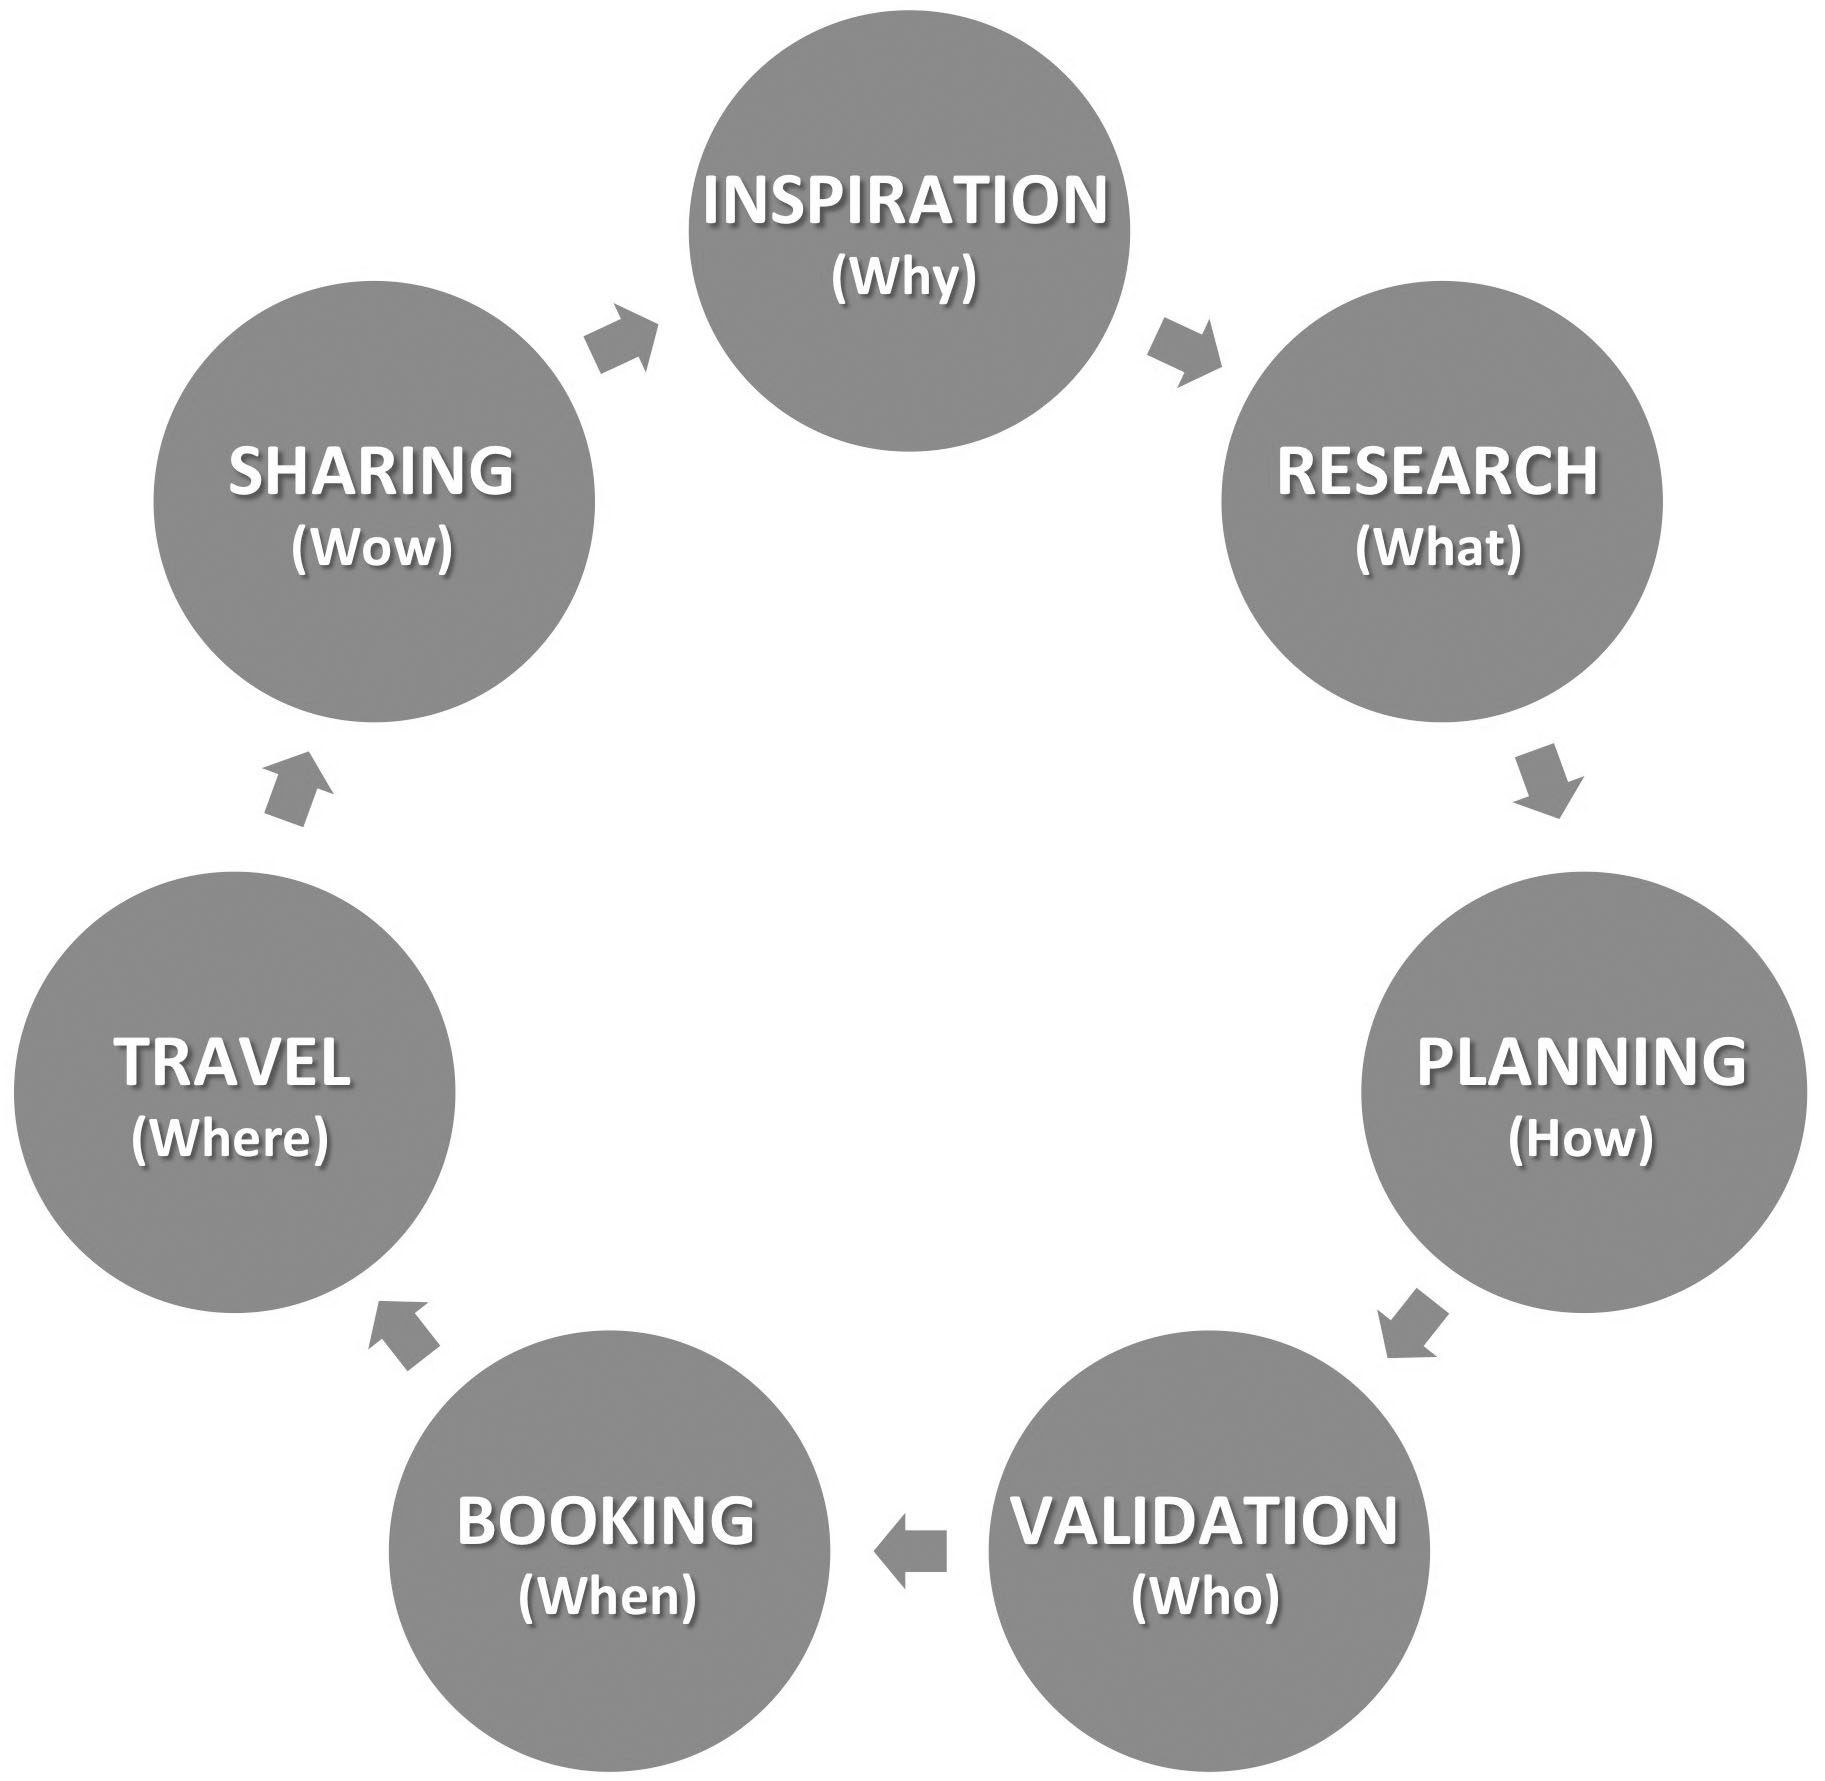
\includegraphics[width=.5\textwidth]{7stages.jpg}
\caption{The Seven Step Travel Process\protect\footnotemark}
\label{pic:sevenstages}
\end{center}
\end{figure}
\footnotetext{\cite{cole:7step}, Seite 8}

% subsection customer_journey_im_tourismus (end)



% section tourismus_und_gastgewerbe (end)

\newpage
\section{Technische Möglichkeiten der digitalen Kontaktaufnahme} % (fold)
\label{sec:technologien}

\subsection{QR Codes} % (fold)
\label{sub:qr_codes}
\buzz{QR Codes} (QR für „Quick Response“) sind zweidimensionale Barcodes, die mit Hilfe von Smartphone–Apps gelesen und ausgewertet werden können. Die quadratischen Elemente des Codes sind in einem ebenfalls quadratischen Muster angeordnet. Neben den eigentlichen Nutzdaten sind im Code auch Muster zur Erkennung der Ausrichtung\footnote{Hierdurch ist die Ausrichtung des Codes beim lesen irrelevant.} sowie Informationen zur Fehlerkorrektur\footnote{Hierdurch wird die Rekonstruktion der Daten selbst bei erheblicher Beschädigung des Codes noch gelesen werden.} enthalten. Die maximale Speicherkapazität beträgt 2953 Byte bei Fehlerkorrekturstufe L (7\%).\footnote{vgl. \cite{iso18004}, Seite 4f}

QR Codes können auch ohne technisches Verständnis kostenlos erstellt\footnote{z.B. \url{http://www.racoindustries.com/barcodegenerator/2d/qr-code.aspx}} und auf Drucksachen jeglicher Art angebracht werden. Der Kunde startet zum lesen der Informationen die entsprechende App auf seinem Smartphone, richtet die Kamera auf den Code. Während des Scans muss das Telefon für etwa ein bis zwei Sekunden still gehalten werden. Nach Abschluss des Scans werden die dekodierten Daten angezeigt, und entsprechende Aktionen können vom Nutzer aus einem Menü ausgewählt werden.\footnote{Etwa der Aufruf einer URL, das Anlegen eines Adressbucheintrags o.ä.} 

\buzz{Denso Wave Incorporated}, die Entwickler und Markenrechtsinhaber der QR Code Technologie,  verlangen keinerlei Gebühren für die Nutzng von QR Codes. Durch Ausnutzung der Fehlerkorrektur ist es möglich, Logos oder andere Grafiken in QR–Codes zu integrieren. Hierdurch kann zwar die Verknüpfung zur eigenen Marke gestärkt werden, allerdings handelt es sich dann nicht mehr um standardisierte QR–Codes. Somit kann es nicht nur zu Leseproblemen sondern auch zu Lizenzforderungen kommen, die sich Denso Wave ausdrücklich vorbehält.\footnote{vgl. \cite{denso-faq}, Nr. 10}
% subsection qr_codes (end)

\subsection{NFC Tags} % (fold)
\label{sub:nfc_tags}
\buzz{NFC} („Near Field Communication“) bezeichnet eine Technologie zur drahtlosen Übertragung von Daten zwischen elektronischen Geräten. Dies können aktive Geräte\footnote{z.B. Smartphones oder stationäre Schreib–Lesegeräte} oder ein aktives Gerät und eine passive Markierung, üblicherweise englisch als \url{Tag} bezeichnet, sein. Der NFC Tag bezieht seine Energie über seine Antenne vom Schreib–Lesegerät. Die theoretisch maximale Entfernung zwischen Sender und Empfänger beträgt 10cm, in der Praxis sind jedoch wenige Millimeter bis ca. 4cm üblich. Die Datenübertragungsrate beträgt hierbei bei maximal 414 Kilobit pro Sekunde. Außer der räumlichen Nähe ist keinerlei vorherige Konfiguration\footnote{wie z.B. das bei Bluetooth notwendige Pairing} notwendig.\footnote{vgl. \cite{nfcforum:about} sowie \cite{google:nfc}, 2:52 Min.}

NFC Tags sind es in verschiedenen Formen und Größen erhältlich. Üblich sind z.B. die Integration in Schlüsselanhänger oder Scheckkarten, aber auch Aufkleber, die an bzw. hinter beliebigen, dünnen Gegenständen platziert werden können. Die Speicherkapazität beträgt zwischen 96 Bytes (Type 1 Tag) und 32 Kilobytes (Type 4 Tag).\footnote{\cite{nfcforum:spec}, Seite 14} NFC Tags können mithilfe eines Smartphones und kostenlos erhältlichen Anwendungen ohne technisches Verständnis beschrieben werden.

Neben Übertragung von Text oder Dateien ist durch NFC auch der Aufruf von Webseiten, die Übergabe von Konfigurations- oder Verbindungsparametern oder die Veränderung von Einstellungen oder das Ausführen von beliebigen, zuvor definierten Anwendungen auf dem Smartphone möglich.

% subsection nfc_tags (end)

\subsection{Bluetooth} % (fold)
\label{sub:bluetooth}

\buzz{Bluetooth} ist eine Technologie zum Aufbau eines \ac{WPAN}, also eines kabellosen, räumlich eng begrenzten\footnote{i.d.R. 10 Meter, jedoch nicht von der Spezifikation beschränkt, vgl. \cite{bluetooth:smart}} Netzwerks. Hierbei werden durch das sogenannte \buzz{Pairing} Geräte miteinander verbunden, ohne dass hierzu weitere Infrastrukturelemente notwendig wären.\footnote{vgl. \cite{bluetooth:spec}, Seite 1, 8} Hierbei werden verschiedene Anwendungsfälle und Geräteklassen durch verschiedene \buzz{Profile} unterstützt.  Die Datenübertragungsrate beträgt hierbei bei maximal 24 Megabit pro Sekunde.\footnote{vgl. \cite{bluetooth:sigv1}, Seite 17f sowie \cite{bluetooth:sigv3}, Seite 277}

Auch wenn komplexere Fälle möglich sind, bestehen typische Bluetooth–Verbindungen beim Endverbraucher zwischen zwei Geräten, meist einem Sender und einem Empfänger. Beispiele hierfür ist der Anschluss von Tastatur und Maus an ein Notebook oder das Abspielen von Musik auf Bluetooth–Lautsprechern. Auch die Übertragung von elektronischen Visitenkarten oder anderen Dateien ist möglich. Die Verbindung wird hierbei auf Betriebssystemebene zwischen den Geräten hergestellt, das Senden wird i.d.R. durch die Auswahl eines entsprechenden Menüpunktes in der jeweiligen Anwendung initiiert. Der Empfänger entscheidet dann per Dialogfenster, ob er die Daten empfangen möchte.

Aufgrund der Vielzahl von Übertragungsprofilen, von denen jedes Gerät nur eine Teilmenge unterstützt kann nicht davon ausgegangen werden, dass jedes Bluetooth–Gerät mit jedem anderen auf die gewünschte Art kommunizieren kann, selbst wenn das Pairing erfolgreich ist.
% subsection bluetooth (end)

\subsection{Bluetooth Low Energy} % (fold)
\label{sub:bluetooth_low_energy}

Das in der Bluetooth Spezifikation 4.0 eingeführte Low Energy Profil (BLE\acused{BLE}) ermöglicht Geräte mit extrem niedrigem Stromverbrauch. Hierdurch sind Anwendungen möglich, welche wie bei der Nutzung von passiven Elementen unabhängig von weiterer Infrastruktur sind, und trotzdem von den Möglichkeiten aktiver Sendern\footnote{z.B. das Senden von Analysedaten oder Messung des Abstands zwischen Sender und Empfänger} profitieren können.\footnote{vgl. \cite{bluetooth:smart}}

BLE Geräte sind auch unter den Markenbezeichnungen \buzz{iBeacon} erhältlich. 
% subsection bluetooth_low_energy (end)

\subsection{Lesbare Internetadressen} % (fold)
\label{sub:kurzlinks}
Die am wenigsten technische Möglichkeit, Kunden auf das digitale Angebot eines Unternehmens hinzuweisen ist die Angabe einer menschenlesbaren\footnote{Lesbar schließt für diese Zwecke auch Piktogramme von bekannten Internetdiensten ein.} \ac{URL}, also Internetadresse\footnote{Obwohl der Begriff URL eine Internetadresse in sehr allgemeiner Form beschreibt, wird er in dieser Arbeit der Lesbarkeit halber synonym zu „WWW–Adresse“ verwendet.} auf Drucksachen. Diese werden vom Kunden in das Smartphone oder in den Webbrowser seines Computers von Hand eingegeben. Je länger diese URL ist, desto schwieriger ist dies.

Daher ist ab einer gewissen Länge bzw. Komplexität der Adresse eine Methode notwendig, mit der diese kürzer bzw. einfacher zu machen. Hierfür stehen kostenlose Internet–Dienste\footnote{z.B. Goo.gl, Ow.ly, FixURL.de oder Bit.ly} sowie Funktionen des \ac{CMS}\footnote{Hier werden kurze, freundliche Adressen wie z.B. \url{http://DieKrone.de/feedback} zur eigentlichen Seite \url{https://secure.holidaycheck.de/hotelbewertung_abgeben.php?action=hotelselect&entityId=161279} weitergeleitet.} zur Verfügung. 
% subsection kurzlinks (end)

\subsection{Nachrichtendienste und Chatsysteme} % (fold)
\label{sub:internet_nachrichtendienste}
Kurznachrichtendienste und Chatsysteme wie z.B. Whatsapp, SMS, Twitter, Facebook–Messenger, iMessage oder Skype können zur digitalen Kommunikation mit Kunden genutzt werden. Die Kommunikationspartner werden hierbei entweder durch Benutzernamen identifiziert, wodurch jedes internetfähige Gerät genutzt werden kann, oder die Kommunikation wird über die Mobilfunknummer der Beteiligen vermittelt, was die Nutzung eines Smartphones notwendig macht, selbst wenn die eigentliche Datenübertragung während der Verbindung über das Internet abgewickelt wird.

Sowohl Twitter als auch Facebook können hierbei nicht nur zur privaten, sondern auch zur öffentlichen Kommunikation genutzt werden.

Aufgrund der hohen Anforderung bzgl. synchroner Kommunikation ist diese Möglichkeit nicht optimal für kleine Betriebe. Die eigentliche Kontaktaufnahme muss zudem über eine der anderen Methoden geschehen. Daher werden Nachrichtendienste und Chatsysteme hier nur der Vollständigkeit erwähnt.
% subsection internet_nachrichtendienste (end)

\subsection{Hotel--Apps} % (fold)
\label{sub:hotel_apps}
Speziell auf das Hotel oder auf das \ac{PMS} zugeschnittene Smartphone–Apps\footnote{z.B. Protel Voyager} ermöglichen durch den Zugriff auf die Daten des Reservierungssystems eine hohe Integrationsstufe und zielgerichtete Kommunikation. Auch sind Funktionen wie die Abfrage von Reservierungs– oder Rechnungsdaten oder Bestellungen beim Zimmerservice möglich.

Die eigentliche Kontaktaufnahme muss zudem über eine der anderen Methoden geschehen, damit der Gast die Anwendung installiert. Des  weiteren richtet sich das Angebot nur an tatsächliche Gäste, nicht wie die anderen hier vorgestellten Technologien auch an Interessenten. Daher werden Hotel–Apps hier nur der Vollständigkeit erwähnt.

% subsection hotel_apps (end)

% section technologische_moglichkeiten_der_digitalen_kontaktaufnahme (end)


\newpage
\section{Bewertungskriterien} % (fold)
\label{sec:kriterien}

Um die verschiedenen technischen Möglichkeiten miteinander vergleichen zu können, bieten sich folgende Kriterien an:

\begin{itemize}
\item Mögliche Quell– und Zielmedien
\item Benötigte Hard-- und Software sowie Infrastruktur auf Seiten des Hotels
\item Anforderungen an das Hotelpersonal bzw. Pflegeaufwand
\item Benötigte Hard-- und Software auf Seiten des Kunden
\item Benutzerfreundlichkeit für den Kunden
\item Bekanntheitsgrad 
\item Verbreitungsgrad 
\item Technische Möglichkeiten\footnote{z.B. Speicherkapazität}
\item Finanzielle Anforderungen\footnote{d.h. die Kosten für ein Exemplar sowie für weitere identische Kopien}
\item Mißbrauchsmöglichkeiten\footnote{z.B. manipulierte Zielmedien}
\end{itemize}

% section bewertungskriterien (end)

